\chapter{Experimental Evaluation} \label{cap:experimental-evaluation}

This chapter distinguishes implemented tooling, exploratory execution, and evidence that could support the research hypothesis. The predecessor snapshot is September 28, 2026, at 00:36 UTC (September 27 in the operator's Pacific timezone); Section~\ref{subsec:h4-snapshot} adds the completed H4 matrix at 01:11 UTC without replacing that historical record. The workflow in Section~\ref{subsec:workflow-stages} governs the transition between these states. A completed training job or a successful engine replay does not by itself constitute a validated comparison.

\section{Experimental Setup} \label{sec:experimental-setup}

The price-download and transformation path, event-feature construction, offline F7 trainers, baseline and hybrid LEAN strategies, decision audit, and analysis commands are implemented. Their existence does not imply that every proposed source or experiment has run. The present pilot uses EUR/USD minute prices and GDELT event intensity. Text sentiment, a real F3 pattern detector, and the proposed broader feature set are absent from this pilot. It must therefore be described as an event-augmented comparison, not as a completed NLP-sentiment study.

The first six available months are allocated to fitting and calibration as shown in Table~\ref{tab:pilot-splits}. The family models use February--June, and logistic stacking uses July. July is not a held-out test for the combined model. The existing trainer also constructs an August test partition, which is excluded from fitting. The initial requested simulation window is September. The start date of February 2 follows from the event feature's one-day publication lag.

\begin{table}[htbp]
\centering
\caption{Chronological allocation for the fixed-model EUR/USD pilot.}
\label{tab:pilot-splits}
\small
\begin{tabular}{p{4.0cm}p{4.0cm}p{5.0cm}}
\toprule
\textbf{Stage} & \textbf{Inclusive dates} & \textbf{Role} \\
\midrule
Family fitting & February 2--June 30, 2015 & LightGBM parameters \\
Combiner calibration & July 1--31, 2015 & Logistic stacking parameters \\
Trainer held-out partition & August 1--31, 2015 & No fitting; not a replay result \\
Initial simulation & September 1--30, 2015 & Frozen-model engine replay \\
\bottomrule
\end{tabular}
\end{table}

Both offline training jobs completed and saved separate portable model artifacts. Each log records 153,531 fitting rows, 32,813 calibration rows, and 30,297 held-out rows, for 216,671 rows in total. These are observation counts, not independent replications. Labels use a fifteen-minute midpoint direction and are purged at split boundaries. The current setup is a single chronological fit, not rolling retraining or CPCV. Additional held-out months can reuse these frozen models; a refit must be registered separately.

In the initial historical pilot, the baseline September replay completed with zero closed trades. Its recorded identifier is \path{baseline/20260927T044836-4cd12c922200}; the UTC identifier falls on September 27 although execution occurred on September 26 in the operator's Pacific timezone. A zero-trade replay requires investigation of coverage, model outputs, and filter vetoes before interpretation. Its zero return and zero-valued summary statistics are not evidence of strategy efficacy or a validated null result. The hybrid replay subsequently completed as \path{hybrid/20260927T053156-4f2ebf081eaf}, also with zero closed trades. Both saved engine files contain the daily equity endpoints for September. Their flat equity cannot estimate return variance or paired uncertainty; the integration check must report unavailable statistics. No paired performance or significance result is claimed here.

Artifacts are kept in the directory \path{2026-09-26-six-month-pilot/} beneath the local \path{algo-suite/data/training/} root. Model JSON files contain split metadata, input hashes, configuration, code revision, and package versions. The job records stage logs and exit status; run directories contain \path{run.json}, \path{trades.json}, \path{metrics.json}, \path{strategy-config.json}, LEAN outputs, and the chain's \path{decisions.parquet}. The repository progress record tracks the initial missing-broker-configuration failure and the resumed OANDA run. These local artifacts must be archived with the final report; a documentation snapshot is not a substitute for them.

The remaining gates are coverage reconciliation for the BigQuery materialization path, point-in-time event availability, execution-cost and risk-economics review, known-answer engine controls, and inspection of decision/trade evidence. Story 11 delivered the corrected inference software of Section~\ref{subsec:rule-significance}; each empirical use of it still requires audited daily equity, cost metadata, actual selection history and block settings registered before evaluation. The wider validation study, additional pairs, and feature ablations remain separate work. The following results are descriptive intermediate observations; unfinished stages remain explicitly unavailable.

\subsection{Snapshot provenance and effective parameters} \label{subsec:intermediate-provenance}

The evidence archive is located beneath the repository root at:
\begin{quote}
\small\ttfamily
algo-suite/docs/stories/in-progress/\\
13-pattern-volume-experiments/evidence/
\end{quote}
The file \path{snapshot-20260928T003601Z.json} records source paths, SHA-256 hashes, code and model identities, job scripts, log excerpts, manifests, and configuration artifacts. The companion \path{per-run-parameters-20260928T003601Z.md} joins each reference R01--R20 to its full run identifier, result, F1--F7 parameter matrix, and per-field provenance. References in the tables and figure legends use these same keys. The clock was confirmed at 00:36:01 UTC; the read-only collection ended at 00:36:02 UTC. It is a bounded snapshot of active jobs, not a claim about their eventual outcomes.

Sixteen run manifests record \path{success=true}; four further runs have live processes but no final manifest. No inspected final manifest records failure. A separate historical failed launch reports a missing \path{broker.adapter}; its result and effective parameters are unavailable. The execution-realism job has completed September and October for both strategies, is running the November baseline, and has not yet started the November hybrid. The A05 sweep has four completed variants and one running variant; the four SpockFX-derived variants have completed. Both annual-protocol simulations are still running. The parallel scripts use bare \path{wait}, so a parent exit code of zero does not establish success of every child; completion here requires each run's own manifest.

The execution-realism and sweep jobs record revision \path{7165308778fd}. Their frozen pilot model hashes begin \path{1a6fd37e96de} (baseline) and \path{a6dda4c2effc} (hybrid). Full revision identifiers, hashes, and training provenance are in the archive. The earlier ungated job records revision \path{709b9bd4bdcf} with uncommitted changes; the pilot hybrid training provenance also carries a dirty revision. Those commit identifiers alone cannot reconstruct the missing patches.

\begin{table}[htbp]
\centering
\caption{Compact parameter reading for execution-model runs R08/R09 (baseline) and R13/R14 (hybrid). The full per-run matrix, including missing historical fields, is in the evidence appendix.}
\label{tab:intermediate-filter-parameters}
\small
\begin{tabular}{p{1.1cm}p{12.2cm}}
\toprule
\textbf{Filter} & \textbf{Archived settings and evidence limits} \\
\midrule
F1 & EMA perception recorded in runtime logs; upstream EMA periods 3/8/60 on minute bars. The 60-period EMA is not an H1/H4 bar series. \\
F2 & RSI period 14, midline 50; MACD 12/26/9, histogram threshold 0. \\
F3 & Bullish: engulfing, hammer, morning star; bearish: engulfing, evening star, shooting star. These configured names do not imply a detector: the predecessor runtime supplies no candle pattern. \\
F4 & Absent from baseline; hybrid event-intensity veto threshold $-0.5$ and sentiment-direction threshold 0.15. Text sentiment is absent in these runs. \\
F5 & Daily/weekly drawdown limits $-0.05/-0.15$; concurrent-trade cap 2; portfolio-at-risk cap 0.10. Configured limits are not independently verified enforcement. \\
F6 & Risk fraction 0.03; swing lookback 60 bars; stop shrink 0.20; minimum 5 pips; minimum reward/risk 2. Target: 2R closes 0.5; trailing step: at 0.5R, stop to $-0.66$R. \\
F7 & Thresholds 0.55/0.45; regime gate off; label horizon 15 minutes. Families: trend, indicator, pattern; hybrid additionally includes news. \\
\bottomrule
\end{tabular}
\end{table}

The same four runs record starting cash 10,000 and shared execution settings: spread 1 pip, commission per lot 0, broker stop level 0, minimum holding bars 0, and \path{close_on_veto=false}. These are archived assumptions, not an economic validation. All fourteen available JSON/YAML configuration pairs agree. The initial and ungated runs R06/R07/R11/R12 lack archived YAML and parameter provenance, and their JSON omits several filter settings; those values remain \textit{missing}, without substitution from current defaults. Running R10 and R19 also lack their own configuration JSON/YAML at this snapshot. A provenance file naming a source is not a substitute for its missing effective values.

\subsection{Annual protocol: training diagnostics and unfinished replay} \label{subsec:intermediate-annual}

The annual job fits family models on March 2--December 31, 2015, calibrates the combiner on January 2016, and constructs a February 2016 held-out partition. Both saved models record 312,878 fitting, 28,802 calibration, and 30,120 held-out rows. Their SHA-256 prefixes are \path{0b41fd39ebf3} and \path{b67ac32e1fc5}; their recorded training revision is the Story 12 revision above. The planned continuous replay spans March 1--October 31, 2016. Baseline R19 and hybrid R20 have no final \path{run.json} or \path{metrics.json}; no annual return is reported. Their full run identifiers and launched arguments are preserved in the appendix.

The saved threshold grid shows descriptive anti-alignment between F7's upward-direction probability and the trend regime. In January, baseline mean probabilities are 0.4791 in bull regimes and 0.5149 in bear regimes; hybrid values are 0.4794 and 0.5148. At thresholds 0.55/0.45, enabling the regime gate leaves only two sell signals for either model, whereas disabling it yields 1,242 baseline and 1,125 hybrid signals. The corresponding ungated label hit rates are 0.569 and 0.564. These are calibration diagnostics over overlapping fifteen-minute labels, not realized trade win rates, independent trials, or proof of profitable anti-trend trading. They do not identify the cause of the replay losses.

The calibration script actually inspects both January and February, including the nominal held-out partition, across eight threshold pairs and both gate settings for each model (64 recorded combinations across the two spans). Thus February is held out from fitting but has already been inspected diagnostically. An untouched-2016-data claim would be false. Any later choice informed by these grids or the ongoing replay must enter the selection history; this snapshot establishes no confirmatory result.

\section{Data Coverage} \label{sec:coverage-results}

\textit{To be added in the final version.}

\section{Baseline Strategy} \label{sec:baseline-results}

The ungated September development replay R07 records 1,032 closed trades and a return of $-0.05\%$ with \path{size=0.5} and \path{cash=10000}. The later execution-model runs use a different sizing and exit contract and record much larger losses (Table~\ref{tab:intermediate-replays}). These are separate experiments on reused historical data; their difference cannot isolate a single execution parameter's effect. The November baseline R10 is still running at the snapshot.

\begin{table}[htbp]
\centering
\caption{Completed execution-model replays, with their own effective parameters linked by R reference to Table~\ref{tab:intermediate-filter-parameters} and the full evidence appendix. Returns and maximum drawdowns are copied from \texttt{metrics.json}; trade counts are from successful \texttt{run.json} manifests.}
\label{tab:intermediate-replays}
\small
\begin{tabular}{llrrr}
\toprule
\textbf{Ref./strategy} & \textbf{Month} & \textbf{Closed trades} & \textbf{Return (\%)} & \textbf{Max DD (\%)} \\
\midrule
R08 baseline & Sept.\ 2015 & 320 & $-52.57$ & 53.8 \\
R13 hybrid   & Sept.\ 2015 & 322 & $-52.75$ & 54.0 \\
R09 baseline & Oct.\ 2015  & 319 & $-53.35$ & 55.2 \\
R14 hybrid   & Oct.\ 2015  & 349 & $-51.37$ & 53.3 \\
\bottomrule
\end{tabular}
\end{table}

The appendix joins each result (R08, R13, R09, R14) to its full run identifier, manifest hash, and model hash. Each month starts separately from 10,000; the months are not presented as a single continuously funded account.

\section{Hybrid Strategy} \label{sec:hybrid-results}

The ungated September development replay R12 records 1,069 closed trades and $+0.51\%$ return under the earlier execution contract. Under the later contract, both completed hybrid replays lose more than half the starting account value, as Table~\ref{tab:intermediate-replays} shows. The baseline--hybrid ordering changes between September and October. Neither ordering supports a news-effect claim without paired inference, audited costs, and the full exploratory selection history.

\begin{figure}[htbp]
\centering
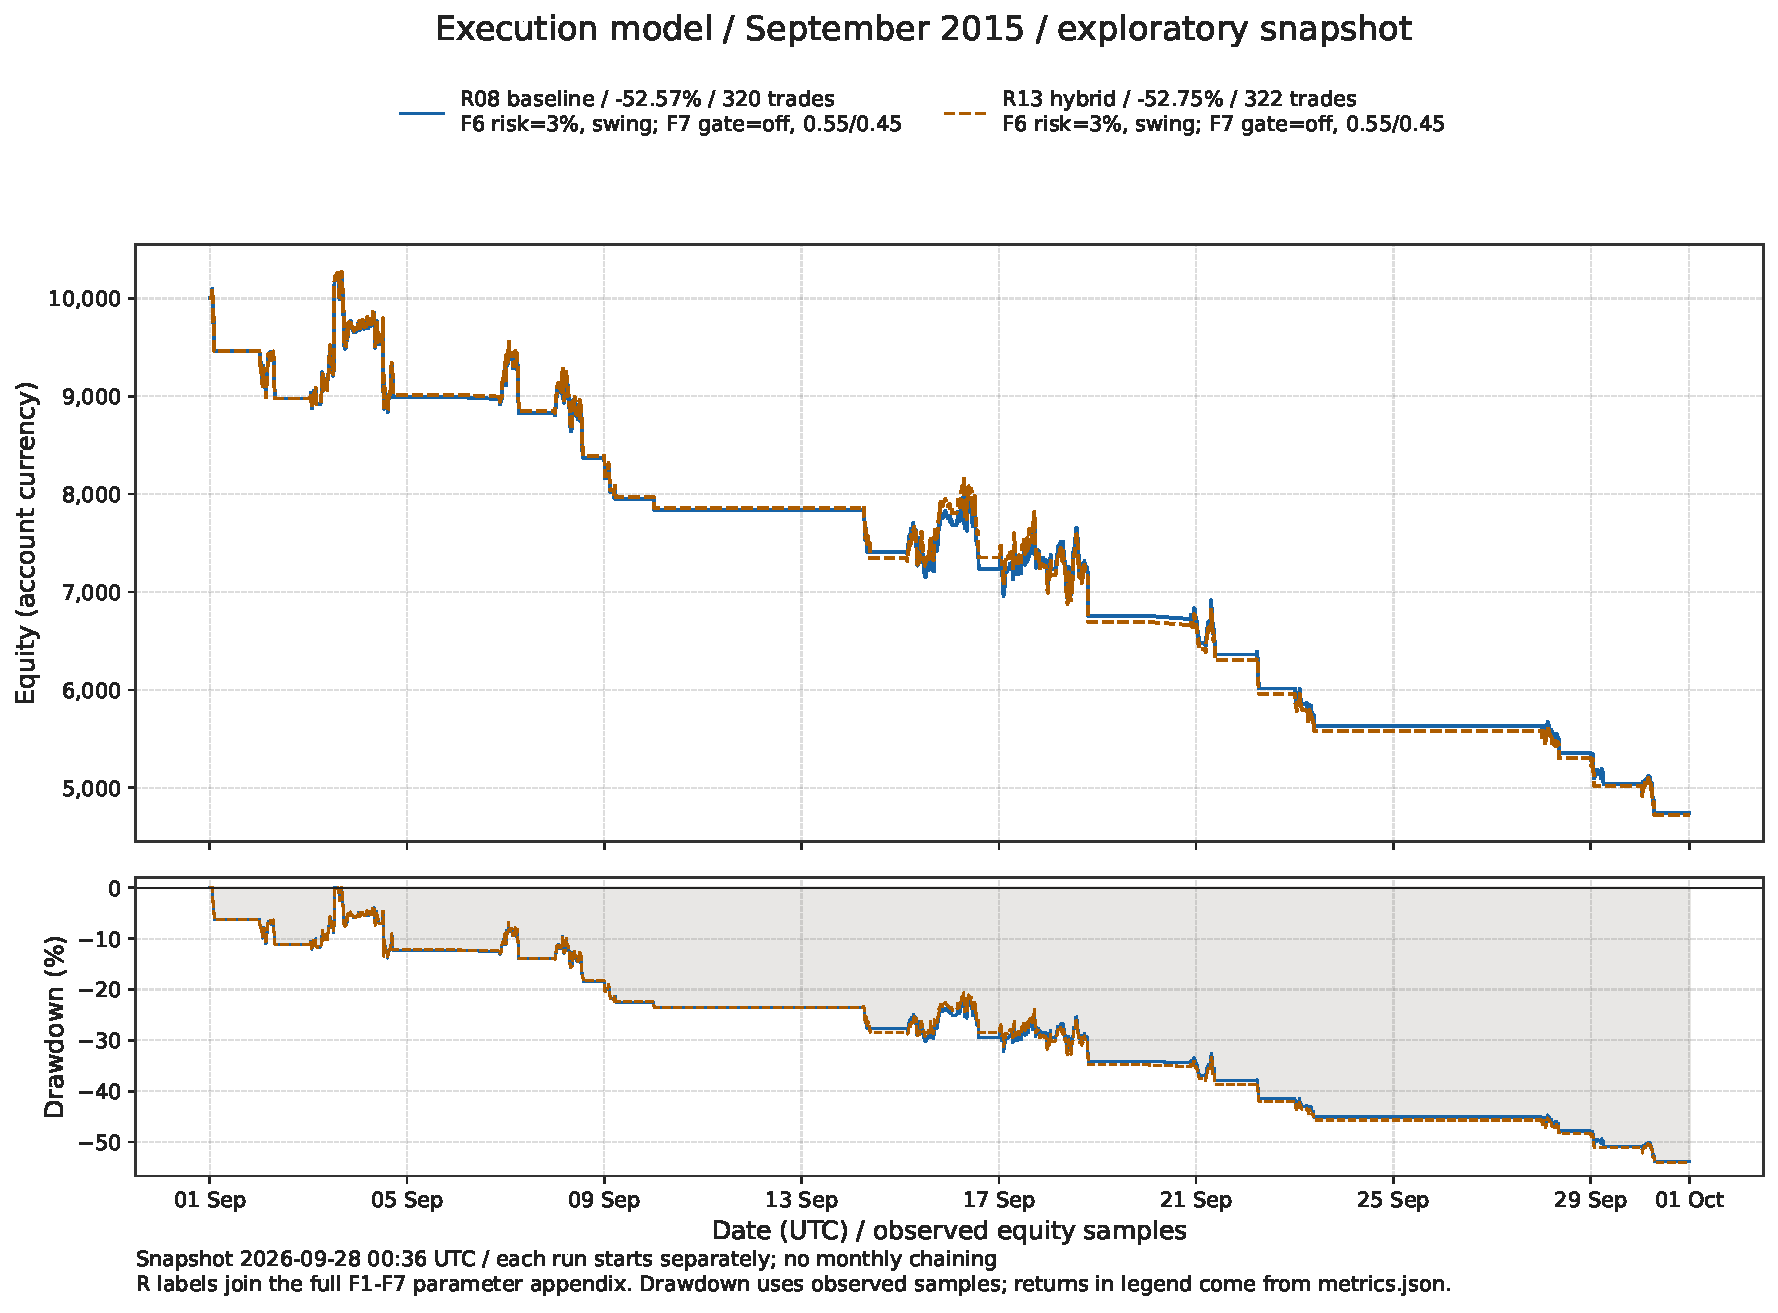
\includegraphics[width=\textwidth]{../algo-suite/docs/stories/in-progress/13-pattern-volume-experiments/evidence/figures/execution-september-print.pdf}
\caption{Observed September equity and drawdown for completed runs R08 and R13, in 2:1 panels. Legends join the parameter appendix; curves use the original \texttt{equity.csv} samples. Drawdown is relative to each sampled running peak and need not equal the engine's rounded maximum-drawdown statistic.}
\label{fig:intermediate-equity}
\end{figure}

Figure~\ref{fig:intermediate-equity} and the October and sweep figures in the evidence archive reuse the repository's equity reader and drawdown calculation. Their presentation adapts the \textit{trading-visualization} skill's Matplotlib layout and styling guidance\footnote{\url{https://github.com/agiprolabs/claude-trading-skills/tree/main/skills/trading-visualization}}; that software guidance supplies no empirical performance evidence. Dark PNG and print PDF variants are provided. No synthetic curve, monthly rebasing, or unfinished annual result is plotted.

\section{Ablations} \label{sec:ablations}

The September sweeps are exploratory parameter comparisons using the frozen pilot baseline model. Table~\ref{tab:intermediate-sweeps} retains losing and zero-trade variants. R02 (a05-gated) remains running with no final result. The full F1--F7 configuration of every listed run, including parameters not varied, is joined to its R reference in the appendix.

\begin{table}[htbp]
\centering
\caption{Completed September-2015 exploratory variants. Every row links its result to its own archived filter matrix by R reference; zero trades do not establish robustness.}
\label{tab:intermediate-sweeps}
\small
\begin{tabular}{llrrr}
\toprule
\textbf{Ref.} & \textbf{Variant} & \textbf{Closed trades} & \textbf{Return (\%)} & \textbf{Max DD (\%)} \\
\midrule
R01 & a05-conservative & 3 & $-0.81$ & 10.8 \\
R03 & a05-risk1 & 552 & $-55.28$ & 55.4 \\
R04 & a05-selective & 6 & $-3.76$ & 5.6 \\
R05 & a05-wide-stop & 14 & $-17.65$ & 21.5 \\
R15 & spockfx-dragon03 & 144 & $-53.47$ & 55.8 \\
R16 & spockfx-dragon03-atr & 437 & $-42.16$ & 50.1 \\
R17 & spockfx-dragon05 & 0 & 0.00 & 0.0 \\
R18 & spockfx-setupnow & 0 & 0.00 & 0.0 \\
\bottomrule
\end{tabular}
\end{table}

The SpockFX labels describe selected plan adaptations, not faithful replications of the reference strategies. At reference revision \path{a1ed6b43b3a7}, \path{deploy.xml} declares a 60-minute selector with a 20\% stop cut and 240-minute deployment templates with a 50\% cut. These H1/H4 settings, indicator-based entry/stop buffers, and strategy rules are not equivalent to the M1 EMA chain and frozen model used in these sweeps. For example, R16 actually archives ATR multiplier 4, stop shrink 0.5, minimum stop 10 pips, and risk fraction 0.01; the YAML comment's ``2 x ATR14'' is not the configured pre-shrink multiplier. Increasing an M1 ATR multiplier does not create H4 candles. Results therefore cannot establish the performance of the original SpockFX system or of the new Story 13 candle/quote-activity implementation.

\subsection{Completed H4 candle and quote-activity matrix} \label{subsec:h4-snapshot}

The second snapshot, clock-confirmed at September 28, 2026, 01:11:14 UTC, contains all four baseline-v1 and four hybrid-v2 Dragon08 H4 swing-proxy cells. Both parent processes record exit 0, both final input checks pass with no errors or mismatches, and all eight individual manifests record success. The interrupted hybrid-v1 root is retained separately: its first two cells succeeded, but its last two logs report ENOSPC before creating their result directories. Its controller-observed parent exit was 1 and its final integrity report is missing. It is not a completed matrix or an additional replication.

The H4 archive joins H01--H08 to each cell's full configuration JSON/YAML, field provenance, model SHA-256, training revision, result manifest, trades, equity, and source fingerprints. Its files, beneath the evidence directory given above, are:
\begin{quote}
\small\ttfamily
h4-snapshot-20260928T011114Z.json\\
h4-parameters-20260928T011114Z.md
\end{quote}
All eight runtime configurations match their prepared JSON, YAML, and model training configuration. The two matrix manifests have identical maps of 249 code-file hashes, despite different recorded Git revisions during concurrent documentation commits. These source fingerprints, not a commit identifier alone, establish the recorded implementation identity.

\begin{table}[htbp]
\centering
\caption{All completed exploratory September-2015 H4 cells. H references join the full per-cell parameter/model appendix; no cell is omitted. Maximum drawdown is the engine-reported statistic.}
\label{tab:h4-results}
\small
\begin{tabular}{lllcrrr}
\toprule
\textbf{Ref.} & \textbf{Family} & \textbf{F3} & \textbf{Volume} & \textbf{Trades} & \textbf{Return (\%)} & \textbf{DD (\%)} \\
\midrule
H01 & Baseline & Disabled & Off & 6 & 1.36 & 5.1 \\
H02 & Baseline & Disabled & On & 3 & 2.87 & 5.1 \\
H03 & Baseline & TA-Lib & Off & 6 & 1.36 & 5.1 \\
H04 & Baseline & TA-Lib & On & 3 & 2.87 & 5.1 \\
H05 & Hybrid & Disabled & Off & 6 & 1.36 & 5.1 \\
H06 & Hybrid & Disabled & On & 3 & 2.87 & 5.1 \\
H07 & Hybrid & TA-Lib & Off & 6 & 1.36 & 5.1 \\
H08 & Hybrid & TA-Lib & On & 3 & 2.87 & 5.1 \\
\bottomrule
\end{tabular}
\end{table}

Closed-trade counts come from both the manifest and the actual trade ledger, not from the reciprocal of a rounded win rate. No new cell has zero closed trades; earlier zero-trade and losing runs remain in the predecessor tables. Equity returns include open-position valuation at the endpoint and are not equivalent to realized closed-trade profit. Identical return rows are not independent replications. Within each volume setting, all four equity CSVs are byte-identical.

\begin{table}[htbp]
\centering
\caption{Effective H4 settings for H01--H08. Every filter is included; the H-keyed appendix repeats the complete resolved matrix and model identity alongside each result.}
\label{tab:h4-parameters}
\small
\begin{tabular}{p{1.2cm}p{12.1cm}}
\toprule
\textbf{Filter} & \textbf{Recorded settings} \\
\midrule
F1 & EMA perception; complete 240-minute bars; EMA 3/8/60. The 60-period series is an H4 EMA, not the reference H1 selector. \\
F2 & RSI 14 with midline 50; MACD 12/26/9 with histogram threshold 0; ATR period 14. \\
F3 & Disabled or TA-Lib per row. Bullish: engulfing, hammer, morning star; bearish: engulfing, evening star, shooting star. \\
F4 & Absent in H01--H04; H05--H08: event veto threshold $-0.5$, sentiment-direction threshold 0.15. Text sentiment is missing. \\
Volume & Absent in odd-numbered H rows; even rows use quote-tick activity, lookback 20 prior closed bars, minimum relative activity 1.0. Not exchange-traded volume. \\
F5 & Daily/weekly drawdown limits $-0.05/-0.15$; concurrent-trade cap 2; portfolio-at-risk cap 0.18. \\
F6 & Risk fraction 0.03; swing lookback 60; stop shrink 0.5; minimum 5 pips; minimum reward/risk 2. Targets 4R/6R, each closes 0.5; trail at 2R to $+0.1$R. \\
F7 & Separate model per cell; horizon 240 minutes; thresholds 0.55/0.45; regime gate off. Trend, indicator, pattern families; hybrid adds news. \\
\bottomrule
\end{tabular}
\end{table}

All cells start with cash 10,000 and record spread 1 pip, commission per lot 0, broker stop level 0, minimum holding bars 0, and \path{close_on_veto=false}. The H4 bar construction and Dragon08 exit settings distinguish these cells from the earlier M1 sweeps, but reference SpockFX entry, stop, trend-buffer, and exit semantics remain replaced by research proxies. Neither faithful replication nor economic validity follows from these settings.

The effective sample is especially small: the controller's completed-bar audit counts 110 September H4 bars, of which the first 59 are consumed by warm-up. Independently inspected decision artifacts contain only 51 decisions per cell, from September 16 at 20:00 UTC through September 30 at 20:00 UTC. Model provenance records 475 fitting, 114 calibration, and 214 test rows; the last count covers August--September and must not be presented as 214 September trading decisions.

\begin{table}[htbp]
\centering
\caption{Decision-level diagnostics, identical across the two families for the counts shown. F4 applies only to hybrid cells.}
\label{tab:h4-diagnostics}
\small
\begin{tabular}{p{8.4cm}rr}
\toprule
\textbf{Observation per cell} & \textbf{Volume off} & \textbf{Volume on} \\
\midrule
Audited decisions / F1 vetoes & 51 / 11 & 51 / 11 \\
Decisions reaching F3 & 40 & 40 \\
Disabled F3: abstentions & 40 & 40 \\
TA-Lib F3: abstentions / buys / sells & 32 / 4 / 4 & 32 / 4 / 4 \\
Hybrid F4: reached / vetoes & 40 / 0 & 40 / 0 \\
Quote-activity vetoes & 0 & 17 \\
Final SELL decisions / closed trades & 40 / 6 & 23 / 3 \\
\bottomrule
\end{tabular}
\end{table}

TA-Lib is not disconnected: F3 records four bearish engulfings, three bullish engulfings, and one hammer among the 40 reached decisions. Baseline F7 probabilities range from 0.408089--0.428667 with detection disabled and 0.408195--0.428762 with TA-Lib. Hybrid ranges are 0.389898--0.436169 and 0.389917--0.436204, respectively. All remain below the fixed SELL threshold 0.45. Pattern and event features change model probabilities without crossing a decision boundary in this sample; identical outcomes therefore do not demonstrate that patterns or news are generally useless. Hybrid F4 records 40 abstentions and no vetoes per cell. The controller's canonical-input audit reports event intensity 0.643298--0.903367, above the $-0.5$ veto threshold, and missing sentiment on all 40 reached decisions; its detailed diagnostic attribution is retained in the evidence synopsis.

\begin{figure}[htbp]
\centering
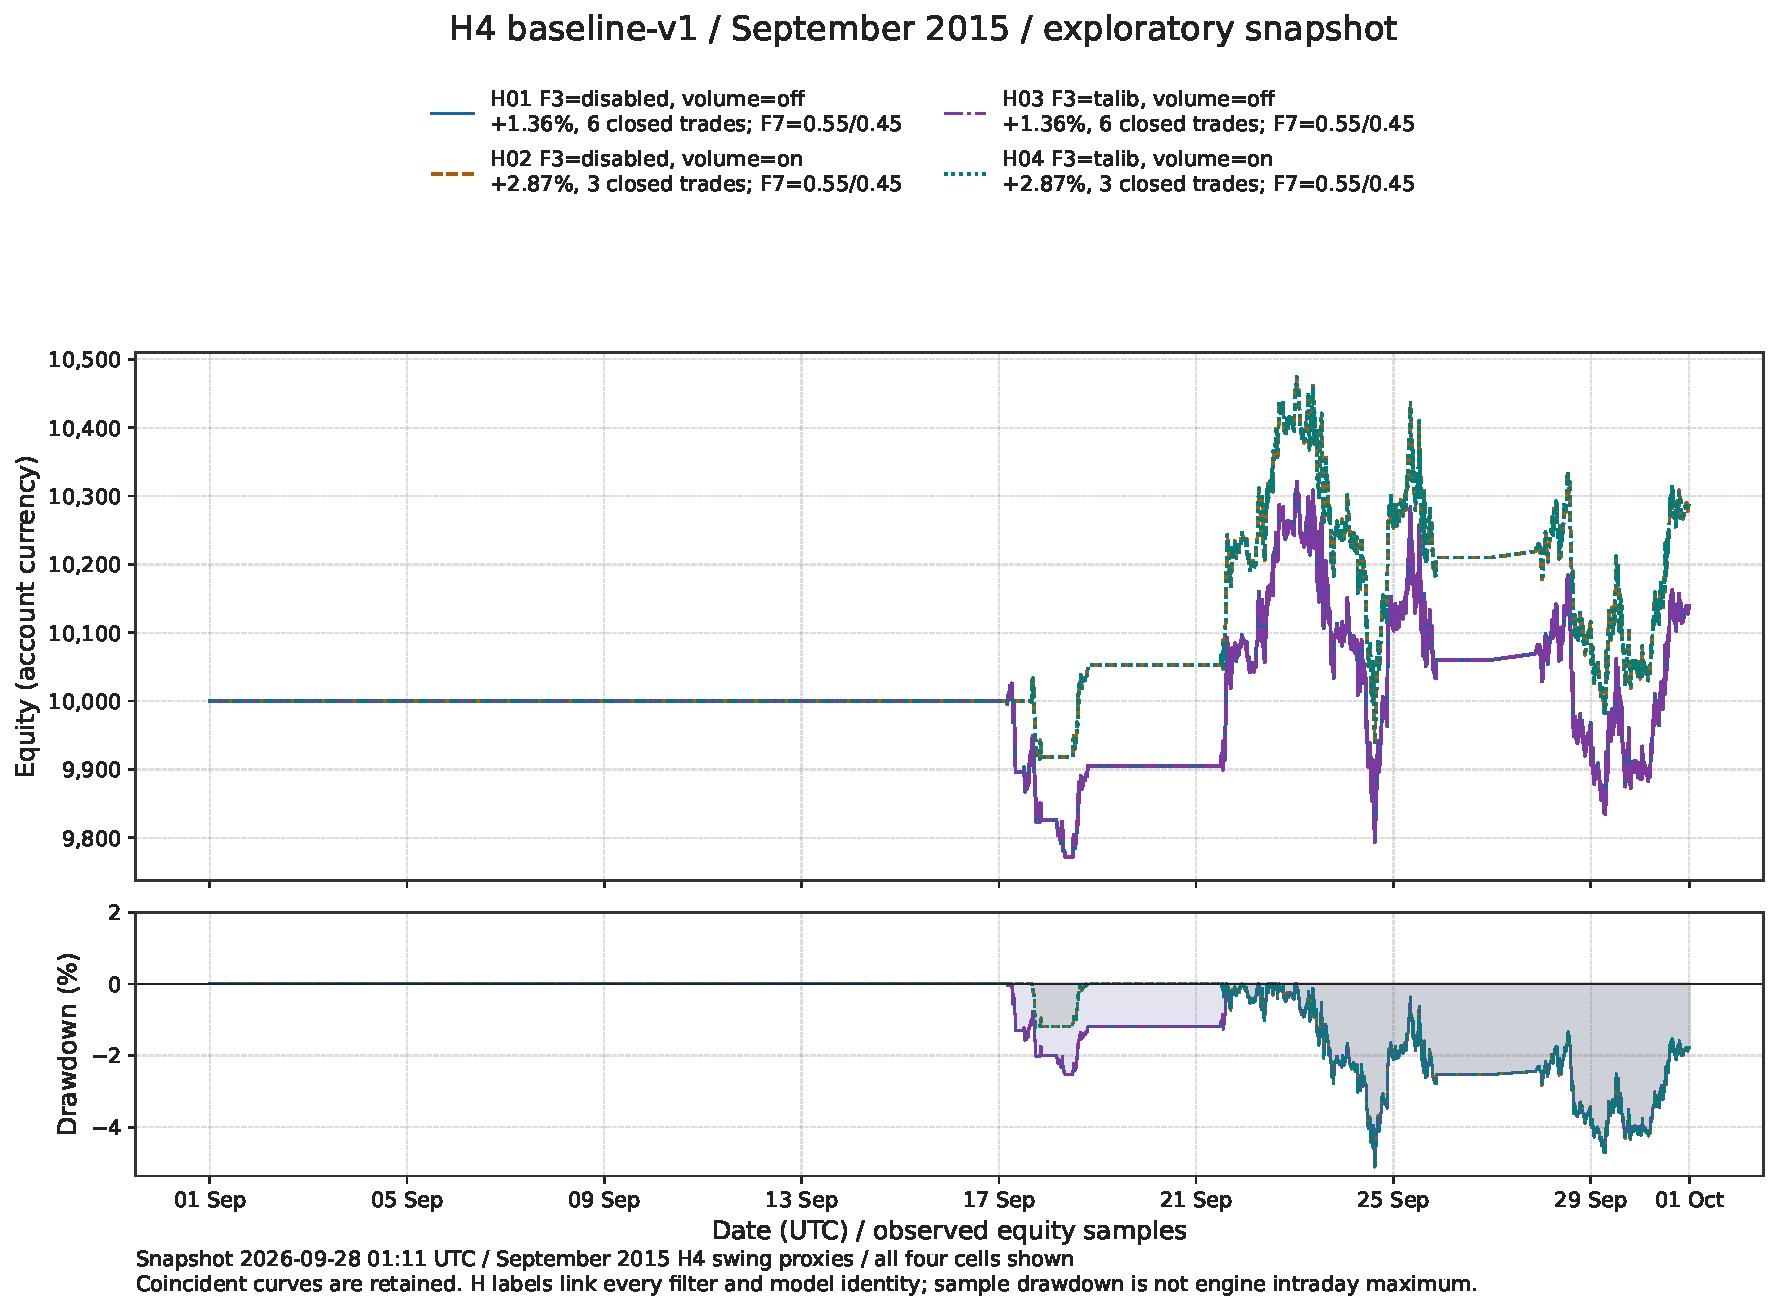
\includegraphics[width=\textwidth]{../algo-suite/docs/stories/in-progress/13-pattern-volume-experiments/evidence/figures/h4-baseline-v1-20260928T011114Z-print.pdf}
\caption{All four baseline H4 cells, including coincident curves. The archive also contains the four hybrid cells and dark-screen variants. Panels use actual equity samples and their drawdown in a 2:1 layout; sampled drawdown need not equal the engine's intraday maximum. Labels join the full parameter appendix.}
\label{fig:h4-equity}
\end{figure}

These favorable H4 observations do not supersede the predecessor losses or calibration anti-alignment. The reused September window, eight separate fitted models, multiple earlier exploratory selections, warm-up truncation, and only three or six closed trades prevent a confirmatory out-of-sample claim. No corrected significance, generalization, causal feature benefit, or economically validated strategy is established.

\section{Comparison with Closest Prior Art} \label{sec:zhang-comparison}

\textit{To be added in the final version.}

\section{Threats to Validity Specific to the Observed Results} \label{sec:experimental-threats}

The present evidence supports an implementation and execution report. It does not establish H1. A short single-pair window, overlapping labels, and daily event values repeated across minute rows limit generalization and invalidate treating row count as an independent sample size. Text sentiment is missing throughout; pattern detection is absent from the predecessor pilot but is observed in the new TA-Lib H4 cells.

Repeated inspection of September, gate changes, threshold grids, execution changes, and nine named sweep variants create multiple exploratory selection opportunities. Selecting the least negative or zero-trade run would not turn this development window into an out-of-sample confirmatory test. The observed losses and F7/regime anti-alignment must be retained alongside favorable historical numbers. The full search history, rather than only the two finally reported strategies, is required for any selection adjustment; the 64 grid entries alone are not an established effective trial count for DSR. Recorded configuration values do not prove effective enforcement, and a successful manifest does not close this economic-validation gap.

The hybrid introduces both a news-family model and an event gate, so a paired difference would represent their combined effect rather than an isolated sentiment contribution. The next-day event lag does not remove the documented late-reporting leakage from aggregation by event date. Fixed stop, pip-value, margin, and risk proxies require economic validation. Finally, schema-v2 inference in Section~\ref{subsec:rule-significance} requires complete daily equity, documented cost treatment and actual selection history. Legacy DSR adjustments and pooled-trade permutation outputs remain exploratory. An unavailable corrected statistic cannot be replaced with a legacy value. Subsequent runs must update this assessment with actual coverage, trade activity, cost assumptions, and paired uncertainty.
